% Chapter Template

\chapter{Haskell Type Checking} % Main chapter title

\label{chap:haskell-type-checking}

\graphicspath{{Figures/HaskellTypeChecking}}

In Chapter \ref{chap:introduction}, we briefly explored the history of programming languages with an emphasis on their practices in type-checking and the paradigms they employ. This chapter focuses closely on Haskell, outlining why it is particularly well-suited for studying improvements in type error detection. We delve into the common techniques for performing type-checking on Haskell programs, specifically the Hindley-Milner type inference system and Algorithm W.

Furthermore, this chapter examines various approaches that have been explored to provide better error messages, including Algorithm M, type error slicing, and interactive debugging. We also discuss key developments in the realm of constraint satisfiability, highlighting their significance in enhancing type error messages. Finally, we revisit the categorization of type errors, this time in light of the aforementioned techniques and tools.

\section{Why Haskell}

Haskell, introduced in 1990, is a functional programming language renowned for its enforcement of pure functional principles, lazy evaluation, and an expressive type system \cite{Hudak2007-kn}. The primary focus of our work is to develop type debugging systems for Haskell that leverage this expressive type system and address its limitations. Although we plan to extend our work to other languages, there are compelling reasons for initially focusing on Haskell.

\subsection*{Haskell In Education}
As discussed in Chapter \ref{chap:introduction}, Haskell plays a significant role in undergraduate computer science education and was designed with this educational purpose in mind. Many textbooks targeting first-year computer science courses and introductions to functional programming recommend Haskell as a pedagogical tool \cite{Bird1998-kv, Davie1992-xv}. Proponents argue that Haskell serves as an ideal platform for teaching programming and rigorous reasoning due to its closeness to mathematical objects. Students often find that Haskell "elegantly admits solutions that are difficult to formulate in imperative languages (minor editing)," a sentiment echoed by computer scientist Edsger W. Dijkstra in a letter advocating for the use of Haskell for freshmen at the University of Texas instead of Java.

Despite the enthusiasm of its advocates, Haskell's actual adoption in universities has been modest. One frequent challenge in teaching Haskell is helping students overcome programming errors \cite{Jun2000-yu, Tirronen2015-nr}. Some recommend using a simplified subset of Haskell's features to avoid the frustrations associated with complex type errors \cite{Heeren2003-kd}. Our research is motivated by both the desire to enhance Haskell's educational value and the real-world challenges associated with teaching the language.

\subsection*{Haskell's special position in programming language research}

Although the full semantics of Haskell have never been formally defined \cite{Hudak2007-kn}, this has not deterred its use as a platform for programming language innovation or for meaningful academic contributions. Subsets of Haskell can be formalized for rigorous language study \cite{FaxEn2002-nd}. Haskell's dual presence in academia and the mainstream programming world uniquely positions it as a testing ground for new programming language features and ideas. Indeed, features such as Haskell's list comprehension have been adopted by languages such as Python and Julia, and its generic type systems have influenced languages such as Java, C\#, and Rust.

Our research in Haskell benefits from the language's relatively small and well-studied specification, enabling rapid implementation of new ideas and swift feedback. We also enjoy support from Haskell's welcoming and active community, which helps guide our efforts towards improved correctness and usability.

\section{Hindley-Milner Type Inference and Algorithm W} \label{sec:hm-inference}

Type inference, also known as implicit typing, is a technique to reduce the number of occurrences of manually ascribing types. Almost all languages today employ a certain level of type inference. For instance, Java versions prior to 10 required users to explicitly declare variable types, which often led to verbosity and redundancy, as shown in Fig.~\ref{fig:example-java}. Java later introduced the var keyword (from version 10 onwards), allowing the type of a variable to be inferred at compile-time based on the assigned value \cite{Java_Developers2023-an}.  

\begin{figure}[hbt]
\centering  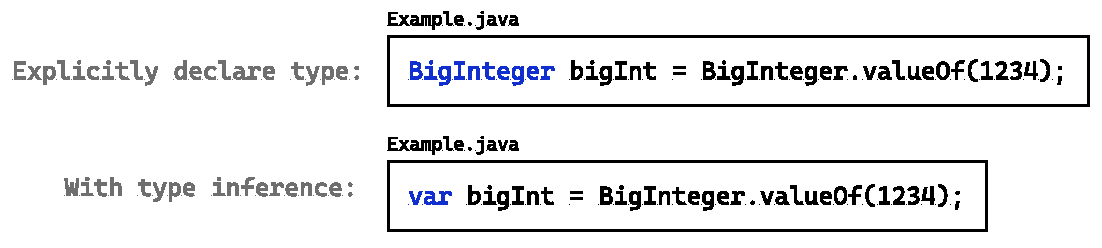
\includegraphics[width=\linewidth]{ExampleJava}
  \caption[An example of a typical Java program with and without using the \texttt{var} keyword]{
    \label{fig:example-java}
      An example of a typical Java program with and without using the \texttt{var} keyword. Before (Top), programmers have to annotate the type identical to the value initializer. After Java 10, this is solved using the local type inference with the \texttt{var} keyword (Bottom).
    }
\end{figure}

In language like Haskell and ML, not only is type inference applied, but its power to detect type error is hugely amplified by the use of the Hindley-Milner type inference  \cite{Damas1982-zw}. The Hindley-Milner Type System, named after its inventors Roger Hindley and Robin Milner, is a type system that can automatically infer the types of expressions in a language with no annotations required. It is a foundational part of the type system in many functional programming languages, including ML, Haskell, and Elm. The system provides polymorphic typing, meaning that a variable can be assigned multiple different types automatically based on its usage context, making it easier to write flexible, reusable code without compromising type safety. In many languages that use this system, it is proven that every expression will be assigned a most general type (principal type) based on its usage. 


In simpler type inference systems, such as the one used in the Java example (Fig.~\ref{fig:example-java}), type inference is local; it occurs within individual assignments, and the compiler may raise errors if it cannot infer types from a single statement. In contrast, the Hindley-Milner system employs a more global approach. It defers type constraint resolution and continues to assess the rest of the program, thereby increasing flexibility and reducing the immediateness of type errors.




\begin{figure}[hbt]
    \centering    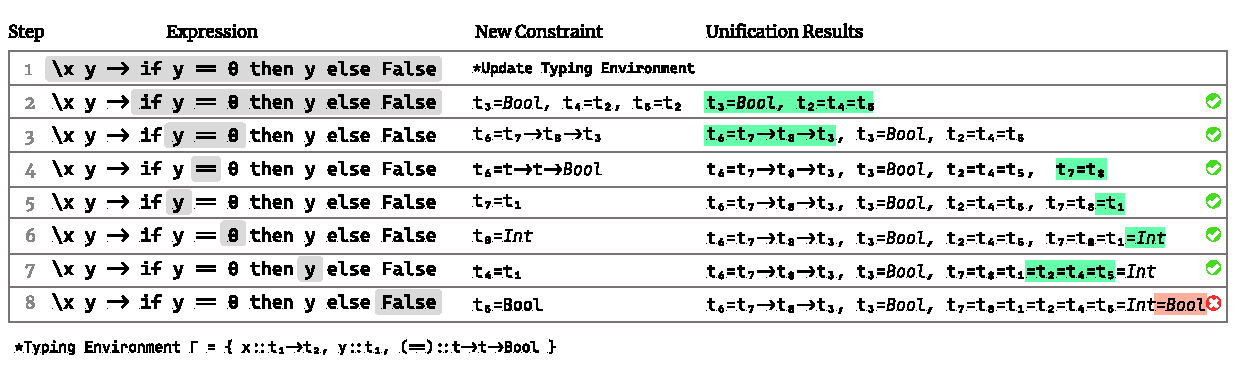
\includegraphics[width=\linewidth]{HindleyMilner}
    \caption[Illustration of Hindley-Milner type checking on a lambda expression]{
      \label{fig:hindley-milner}
      Illustration of Hindley-Milner type checking on a lambda expression. Initially (Step 1), fresh type variables $t_1$  and $ t_2 $ are introduced to assign types to $x :: t_1 \to t_2$ and $y :: t_1$, with $ t_2$ serving as a placeholder for the expression’s right-hand side. It then examines the right-hand side 'if' expression, creating three additional variables: $t_3$ for the condition, and $t_4$ and $t_5$ for the left and right branches, respectively. Unification constraints are then applied, stipulating $t_3$ as a boolean $Bool$, and requiring $t_4$ and $t_5$ to match $t_2$. The process continues traversing the syntax tree until Step 8, where a type mismatch occurs as $t_5$, previously unified with an integer type, is attempted to be unified with a boolean type, leading to a type inference error.
       }
\end{figure}

This sophisticated type inference mechanism found in the Hindley-Milner system underpins its wide adoption in the realm of functional programming. It exemplifies a shift towards more intelligent compilers that enhance developer productivity and code maintainability by abstracting the complexities of explicit type management.

\textbf{Algorithm W}  The foundational mechanism of the Hindley-Milner type system is Algorithm W, a method to deduce the most general types for each expression in programming languages that support polymorphic types. This algorithm starts by assigning a unique type variable to each expression. It then recursively analyzes the structure of the program, generating a set of type constraints by inspecting each syntax node—as shown in Fig.~\ref{fig:hindley-milner}. This process involves the creation of new type variables and the unification of these variables with others or with specific types.

Unification is a critical step: It attempts to make different type variables agree by finding a common type that satisfies all constraints. If unification is unsuccessful at any point, the type-checking process halts immediately, indicating a type error. The algorithm reports the expression where the last constraint was produced, but this is often reported as the sole source of the error.

Despite the seismic influence of type theory and the conciseness of the programming style it helps achieve,  the Hindley-Milner type system can be challenging in terms of usability. One notable drawback is how it handles error reporting. When type inference fails, the error messages can be cryptic and difficult to interpret. This is because the algorithm typically reports only the final constraint that led to the failure, omitting earlier but potentially relevant constraints. Unlike simpler cases in languages like Java, where a type error might be isolated to a single line, in a Hindley-Milner-based system, the underlying issue could be located anywhere in the program. This often leaves programmers scanning extensive sections of code to identify the root cause of the error. 

This aspect of Algorithm W highlights a trade-off between the power of the type inference offered by the Hindley-Milner system and usability, notably in terms of error diagnostics and clarity. This has prompted ongoing research into improving error reporting in systems based on this algorithm, seeking to make them more accessible and easier to use for programmers.

\textbf{Algorithm M} 
In response to the usability challenges posed by Algorithm W, an alternative approach known as Algorithm M was proposed \cite{Lee1998-fx}. This method modifies the direction of type inference from a bottom-up to a top-down process. By carrying constraints from the outer structure of the program to the substructures, Algorithm M allows for more contextual analysis, resulting in more intuitive error messages in certain scenarios, as illustrated in Fig.~\ref{fig:algorithm-m-1}. 

\begin{figure}[hbt]
  \centering
  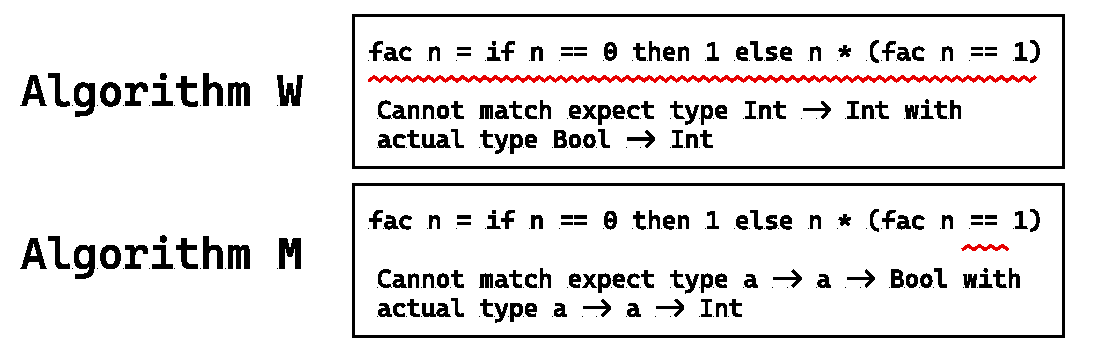
\includegraphics[width=0.8\linewidth]{AlgorithmWM1.pdf}
  \caption[Comparison of error reporting between Algorithms M and W]{
    \label{fig:algorithm-m-1}
    Comparison of error reporting between Algorithms M and W. In this example, Algorithm M identifies a more precise and plausible error location, whereas Algorithm W only provides a general, less specific error location.}
\end{figure}


\begin{figure}[hbt]
\centering  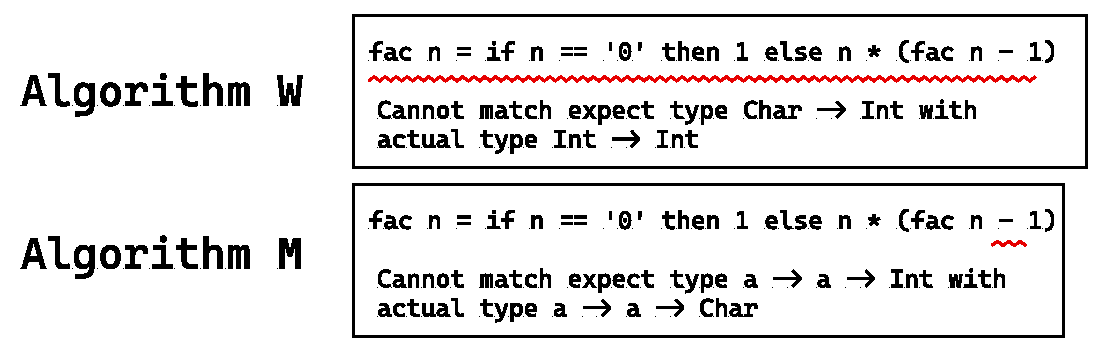
\includegraphics[width=0.8\linewidth]{AlgorithmWM2}
  \caption{
    \label{fig:algorithm-m-2}
    Analysis of error detection where Algorithm M fails to identify the correct error location, suggesting that \texttt{'-'} is causing the error. Despite this, Algorithm W continues to provide a general, less specific error location.}
\end{figure}


Despite its improvements in some cases, Algorithm M does not consistently outperform Algorithm W in terms of error clarity and can still produce misleading results, as shown in Fig.~\ref{fig:algorithm-m-2}. Both algorithms essentially face the same fundamental limitation: type inference is conducted step-by-step through unification, and once constraints are unified, they are discarded and unretrievable. Consequently, errors detected by these algorithms may not accurately reflect the root issues if multiple possible causes of types exist.

A lesson that can be learned from both Algorithm W and M is the recognition that no inference method ensures that it will perfectly align with the programmer’s intentions. Rather than ambitiously pinpointing where the root cause may lie, a more realistic goal might be to represent type errors succinctly without making assumptions.


\section{Type Error Slicing}

Type error slicing is an advanced technique intending to enhance the meaningfulness of type error messages provided to programmers. This approach, referenced in works by Tip and Dinesh~\cite{Tip2001-qn} and Haack and Wells~\cite{Haack2004-fr}, improves upon traditional type inference methods by postponing the unification process until all relevant constraints have been established. Type error slicing incorporates two principal innovations:


\begin{enumerate}
  \item {
    \textbf{Labeled Constraints:}
    This involves assigning identifiable labels to constraints based on their locations within the program. These labels are subsequently used to trace and diagnose parts of the code associated with a type error, offering clearer insights into the origins of an error.
  }
  \item {
    \textbf{Minimal unsatisfiability analysis:} 
    This technique focuses on identifying the smallest set of conflicting constraints that cannot be satisfied simultaneously. This means finding the necessary evidence needed to reproduce the failed unification, but nothing more than that. This approach significantly improves the diagnosis of type errors by avoiding the biases found in both Algorithms W and M.
  }
\end{enumerate}


\begin{figure}[hbt]
  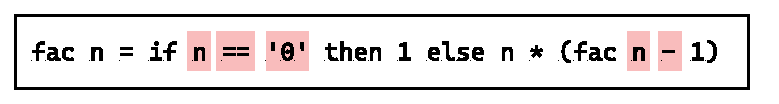
\includegraphics[width=0.8\linewidth]{TypeErrorSlicing.pdf}
  \caption[Illustration of type error slicing applied to the Haskell function \texttt{fac}]{
    \label{fig:type-error-slicing}
    Illustration of type error slicing applied to the Haskell function \texttt{fac}. The highlighted "slices" indicate conflicting type inferences for the variable \texttt{n}: it is inferred as \texttt{Char} since it is compared against \texttt{'0'}, yet it must be an integer because it is used in arithmetic subtraction. This conflict leads to the identification of a type error.}
\end{figure}

In contrast to conventional methods, type error slicing provides a comprehensive view of error locations, as demonstrated in Fig.~\ref{fig:type-error-slicing}. It allows programmers to understand type errors more thoroughly by presenting both sides of typing conflicts. It has less chance of missing critical clues, thus facilitating a more informed debugging process.

Over time, type error slicing has become a preferred method for optimizing type errors in research. Innovations in this area include more efficient methods of finding minimal unsatisfiable subsets \cite{Liffiton2008-mx, Bailey2005-hi, Bacchus2015-of}. Type error slicing has also been enriched by exploring various underlying constraint languages to encode more complex type system features, such as those using SMT (Satisfiability Modulo Theories) \cite{Pavlinovic2015-ke} and Constraint Handling Rules \cite{Stuckey2003-pz}. These advancements have broadened the scope and applicability of type error slicing, making it a valuable tool for programming language development and error diagnosis.


\section{Interactive Type Debugging}

Traditional type error slicing methods have been instrumental in localizing type errors by highlighting a comprehensive yet minimal set of related code locations. Despite the advantages, there are several key limitations associated with the localization and diagnosis in type error slicing:

\begin{figure}[hbt]
  \centering
  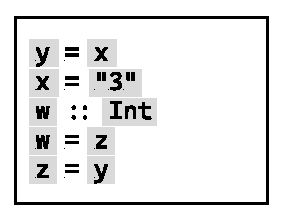
\includegraphics[width=0.4\linewidth]{SlicingCounterExample}
  \caption[An example where type error slicing is less useful, highlighting every possible location in the source code]{
    \label{fig:slicing-counter-example}
      In this case, type error slicing is less useful, highlighting every possible location in the source code.}
\end{figure}

\begin{enumerate}
  \item {
    \textbf{Limited Code Reduction:} Although MUS-based error slicing can effectively narrow down the potentially defective code areas, studies such as Binkley's empirical analysis on program slicing \cite{Binkley2007-ev} suggest that this method only reduces about 30\% of the code that needs to be examined to understand a type error. The minimal nature of MUS often prevents further reduction, which can be insufficient for complex errors, as demonstrated in Fig.~\ref{fig:slicing-counter-example}, where virtually every location in the program could be implicated in the error.
  }

  \item{
    \textbf{Lack Of Enhanced Information Encoding:}  The existing MUS-based approaches might highlight critical error sites, but they often fail to capture the breadth of information required to fully understand and resolve type errors, especially in systems with complex type features.
  }
\end{enumerate}

To address these limitations, pioneering tools such as Chameleon \cite{Stuckey2003-pz} have been developed. Initially introduced in the early 2000s, Chameleon served as a command-line tool aimed at improving type error reporting within the Haskell programming language. Unlike typical type-error slicing methods, Chameleon utilizes a more expressive constraint language, the constraint handling rules (CHR), which enables the support of more flexible relational constraints tailored to advanced type-level features such as type classes and functional dependencies.

A key innovation of Chameleon is its adoption of interactive type debugging. This approach not only identifies potential error locations, but also reveals that there could be multiple sets of potential types, most general unifiers, that could resolve the type issues present in the erroneous program. These types can be traced to distinct sets of code locations.

With interactive type debugging, programmers can query the type information of any possible resolution, effectively allowing programmers to ask counterfactual questions such as ``what would the type of the expression be if the type error is fixed". This interactive process significantly advances the programmers' understanding of type errors by allowing them to explore different resolution paths and better comprehend the type system's behaviors and expectations.

Interactive type debugging thus represents a significant evolution in the handling of type errors, offering a more dynamic and informative approach compared to static slicing methods. This development underscores a shift towards more user-centered diagnostic tools in programming, where clarity and interactivity play vital roles in problem-solving.

\begin{figure}[hbt]
  \centering
  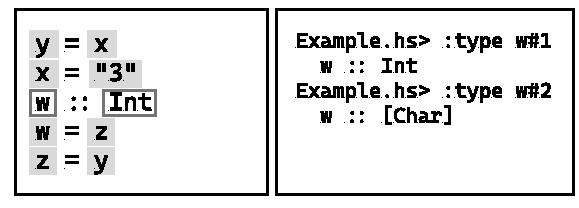
\includegraphics[width=0.8\linewidth]{ChameleonInteractive}
  \caption[Demonstration of the interactive debugging feature in Chameleon]{
    \label{fig:chameleon-interactive}
    Demonstration of the interactive debugging feature in Chameleon. The source code is highlighted in two distinct styles (solid and outline), suggesting two potential types assignable to the variable \texttt{w} (left). Complementary details about these types are further explored through a command line query interface (right). }
\end{figure}

\section{The Analysis of an Unsatisfiable System}

A slicing-based approach benefits significantly from the established tools and techniques in constraint satisfiability. Key instruments in this domain include the Minimal Unsatisfiable Subset (MUS), the Minimal Correction Subset (MCS) and the Maximal Satisfiable Subset (MSS).

\subsection*{Minimal Unsatisfiable Subset}

The MUS is a widely used tool in programming error analysis; it is used in various programming slicing tools \cite{Haack2004-fr, Pavlinovic2015-ke, Stuckey2003-pz}. The MUS represents the smallest possible subset of a constraint system that still remains unsatisfiable, meaning that no values can be assigned to the logical variables without causing a conflict. This subset is crucial in determining the minimal set of code locations responsible for a type error.


Formally, a minimal unsatisfiable subset (MUS) $M$ of a constraint system $C$ is a subset $M \subseteq C$ such that $M$ is unsatisfiable and $ \forall{c} \in M : M \setminus \{c\}$ is satisfiable.  An MUS provides a concise explanation for the infeasibility of a system, highlighting a logical pathway from one conflicting location to another. Thereby, MUS is often associated with addressing the "Why not" question \cite{Ignatiev2020-xu, Nelson2017-ar}, in other words, finding the minimal contributors that prevent the system from emitting a certain behavior (in our case, such behavior is to become well-typed).

It is important to note that an unsatisfiable constraint system may contain multiple MUSes. For instance, consider a system with 5 propositional constraints depicted in Fig.~\ref{fig:mus-example} - the system is infeasible as a whole. Within it, three MUSes can be identified. Each MUS is minimal, since removing any single constraint results in a satisfiable system. Typically, an incremental algorithm is employed to discover a single MUS. This algorithm starts from an empty set and adds one constraint at a time until the set is no longer satisfiable, indicating that the last added constraint must be an element of the MUS. 

\begin{figure}[hbt]
  \centering
  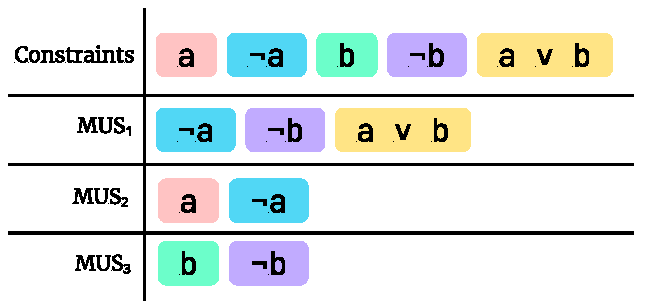
\includegraphics[width=0.8\linewidth]{MUS}
  \caption[An illustration of Minimal Unsatisfiable Subsets (MUSes)]{
    \label{fig:mus-example}
    An example of a constraint system modeled in propositional logic featuring 7 constraints and 2 logic variables \texttt{a} and \texttt{b}. The system is initially infeasible.  Three potential Minimal Unsatisfiable Subsets (MUSes) can be identified. Each MUS is itself unsatisfiable. More critically, the removal of any single constraint from an MUS yields a satisfiable set of constraints. }
\end{figure}

\subsection*{Minimal Correction Subset and Maximal Satisfiable Subset}

Beyond the MUS, the Minimal Correction Subset (MCS) represents the smallest group of constraints that, when removed, resolves the infeasibility (defect) of the system. Formally, a minimal correction set (MCS) $M$ of a constraint system $C$ is a subset $M \subseteq C$ such that $C \setminus M$ is satisfiable and $\forall{S} \subset M : C \setminus S$ is unsatisfiable. This "correction" subset is crucial for identifying the minimal changes needed to rectify errors in a program. Thus, MCS is often associated with addressing the ``Why" question \cite{Ignatiev2020-xu, Nelson2017-ar}, in other words, finding the minimal reasons that trigger a certain behaviour. In the example (Fig.~\ref{fig:mcs-example}), 4 MCSes can be found. Removing each of these will result in a satisfiable set of constraints. Note that the satisfiability of MCSes themselves is not important.  


\begin{figure}[hbt]
  \centering
  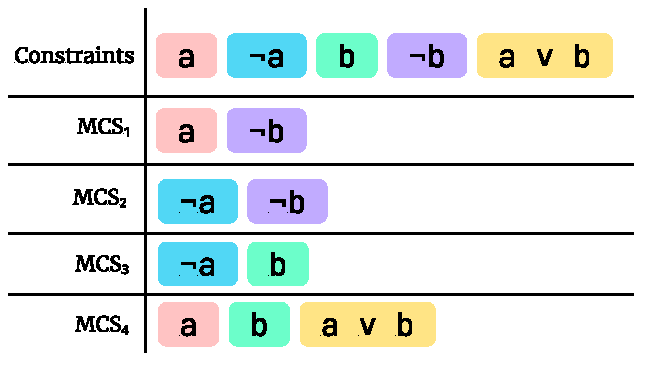
\includegraphics[width=0.8\linewidth]{MCS}
  \caption[An illustration of Minimal Satisfiable Subsets (MCSes)]{
    \label{fig:mcs-example}
    Depiction of a constraint system in propositional logic, consisting of 7 constraints and 2 logic variables \texttt{a} and \texttt{b}. Initially, this system is infeasible. Four Minimal Satisfiable Subsets (MCSes) can be identified, where the removal of each individual MCS from the constraint system leads to a maximally feasible system.}
\end{figure}

The Maximal Satisfiable Subset (MSS) is the complement of an MCS. A maximal satisfiable subset (MSS) $M$ of a constraint system $C$ is a subset $M \subseteq C$ such that M is satisfiable and $\forall{c}\ in\ C \setminus M:M\cup\{c\}$ is unsatisfiable. In practical terms, an MSS represents the largest portion of the constraint system that does not contribute to the type error, offering insights into the potential outcome of a working system after removing the defect. An example of MSSes in a constraint system can be seen in Fig.~\ref{fig:mss-example}.




\begin{figure}[hbt]
  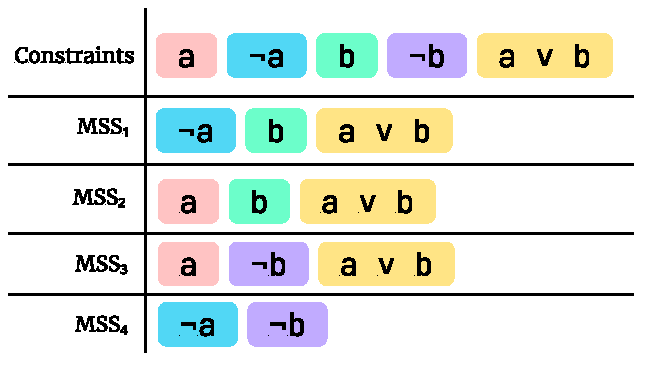
\includegraphics[width=0.8\linewidth]{MSS}
  \caption[An illustration of Maximal Satisfiable Subsystems (MSSes)]{
    \label{fig:mss-example}
    Depiction of a constraint system in propositional logic with 7 constraints and 2 logic variables \texttt{a} and \texttt{b}. While the full system is infeasible, four Maximal Satisfiable Subsystems (MSSes) are found. Each MSS is satisfiable in itself, but including any additional constraints from the system renders it unsatisfiable. }
\end{figure}

\subsection*{MUS Enumeration}

Since a system can harbor multiple MUSes and MCSes, enumerating these subsets reveals a deeper understanding of the different conflict sources and potential correction plans. Enumerating MUS/MCS is crucial for the comprehensive analysis in program fault detection~\cite{Bekkouche2015-is}, circuit design~\cite{Gaber2022-te}, and explaining machine learning models \cite{Marques-Silva2023-nk}.

However, MUS enumeration is inherently challenging due to its computational demands. The most naive approach to finding all MUSes is to exhaust the power set of the constraint system, which is impractical for large systems. Advanced algorithms like MARCO~\cite{Liffiton2016-xi} and MUST~\cite{Bendik2020-pz} utilize heuristics to avoid traversing large blocks of subsets, enhancing efficiency and making the process viable even for complex systems.

This analysis forms a foundational aspect of our discussions on our type error debugging system in Chapter \ref{chap:goanna}, providing a structured approach to tackling programming errors through the lens of constraint satisfiability.

\section{Categories of Type Error}

Building upon the introduction of the Minimal Unsatisfiable Subset (MUS) discussed earlier, we revisit and refine the 3 categories of type errors proposed in Chapter \ref{chap:introduction}. This categorization directly relates to the constraint representations of type errors and the number of MUSes found within the system. This connection aims to bridge the gap between the intuitive debugging approaches of human programmers and the formal analysis offered by constraint satisfiability.

\subsection*{Multi-step Type Error}

\begin{figure}[hbt]
  \centering 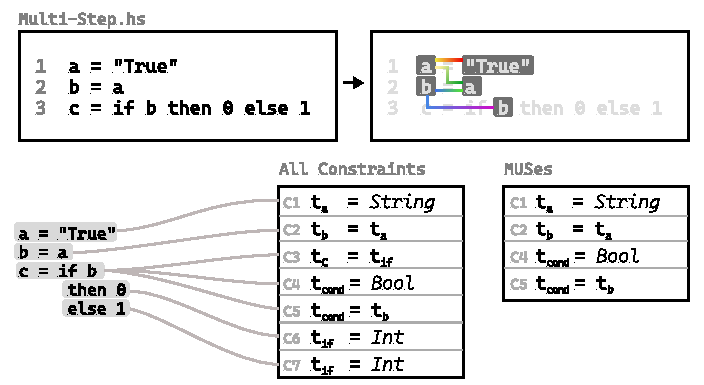
\includegraphics[width=\linewidth]{Multi-Step-MUS}
  \caption[Illustration of a multi-step type error in the context of MUSes]{Illustration of a multi-step type error influenced by potential issues in the definition of \texttt{a}, \texttt{b}, or the conditional expression involving \texttt{b}. These elements are logically connected as depicted (Top Right). The analysis of the source code yields 7 constraints (Bottom Left), from which only one Minimal Unsatisfiable Subset (MUS) is identified (Bottom Right).}
  \label{fig:multi-step-2}
  \end{figure}


Multi-step type errors involve a sequence of logical deductions that link one conflicting location to another. When viewed as constraint system, a multi-step type error is a type error contains a single MUS. Relaxing any constraint within the MUS leads to a satisfiable system, implying that each location correlated to a constraint in the MUS could potentially cause the type error. For instance, in Fig.~\ref{fig:multi-step-2}, the MUS consists of the constraints $\{C1, C2, C4, C5\}$. Removing any one of the elements would allow the program to type-check successfully.

\subsection*{Multi-witness Type Error}

\begin{figure}[hbt]
    \centering
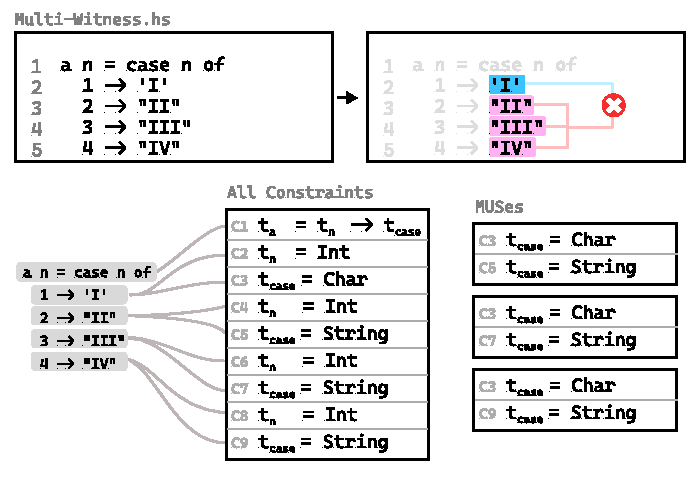
\includegraphics[width=\linewidth]{Multi-Witness-MUS}
  \caption[Illustration of a multi-witness type error in the context of MUSes]{\label{fig:multi-witness-2}
  Analysis of a multi-witness type error, where the \texttt{case} expression could be interpreted as type \texttt{Char} or \texttt{String}. This scenario showcases a type disagreement with three witnesses against one witness (Top Right). From the source code, 9 constraints are established (Bottom Left), resulting in 3 identified MUSes. Interestingly, all MUSes include constraint C3, suggesting its pivotal role in favoring the possibility that the \texttt{Char} type is erroneous.}
  \end{figure}

A multi-witness type error occurs when multiple locations (witnesses) on one side of a conflict suggest the same type assignment. When viewed as a constraint system, a multi-witness type error contains multiple MUSes. The precise number of MUSes depends on the number of witnesses at each endpoint. If a type error involves $m$ witnesses on one side and $n$ on the other, there will be a total of $m \times n$ MUSes. For example, in Fig.~\ref{fig:multi-witness-2}, there are three MUSes: $\{C3, C5\}, \{C3, C7\}, \{C3, C9\}$. It is crucial to note that the constraint C3 appears in every MUS, signaling a likely root cause.

\subsection*{Multi-party Type Error}

\begin{figure}[hbt]
  \centering
  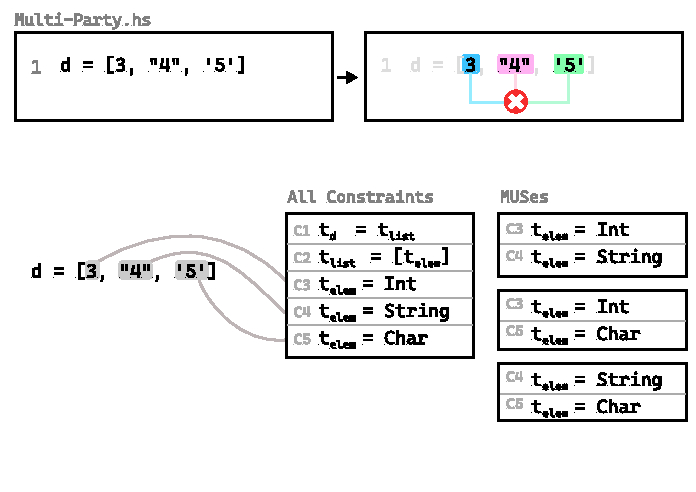
\includegraphics[width=\linewidth]{Multi-Party-MUS}
  \caption[Illustration of a multi-party type error in the context of MUSes]{\label{fig:multi-party-2} Analysis of a multi-party type error regarding the list \texttt{d}, which could alternately be typed as \texttt{[Int]}, \texttt{[String]}, or \texttt{[Char]}. The conflict is depicted as a disagreement among three parties (Top Right). An analysis based on the source code generates 5 constraints (Bottom Left), leading to 3 distinct Minimal Unsatisfiable Subsets (MUSes). Notably, this scenario differs from the multiple witness type error as no single constraint appears across all MUSes.}
  \end{figure}

A multi-party type error features several irreconcilable type assignments stemming from different locations within the source code. Like multi-witness errors, multi-party errors contain multiple MUSes. In the example shown in Fig.~\ref{fig:multi-party-2}, there are three MUSes: $\{C3, C4\}, \{C3, C5\}, \{C4, C5\}$. Unlike the multi-witness scenario, no single element appears across all MUSes, suggesting a more complex type conflict scenario.

These categories of type errors illustrate the main challenges in explaining type errors effectively:
\begin{enumerate}
  \item {
    \textbf{Multi-step Type Errors:} It is beneficial to clarify the interdependent relationships between each pair of constraints sharing the same logical variable.
  }
  \item {
    \textbf{Multi-witness Type Errors:} Identifying the number of witnesses and their associated source code locations on each side of the conflict can be insightful.
  }
  \item {
    \textbf{Multi-party Type Errors:} Breaking down these errors into simpler forms can aid in understanding and resolving them.
  }
\end{enumerate}

It is important to recognize that these categories are not mutually exclusive; a type error may exhibit characteristics from multiple categories, necessitating a combination of approaches to fully elucidate the underlying issues.

\section{Conclusion}

This chapter began by establishing a historical context for Haskell, highlighting its significant role in both educational settings and programming language research. We explored various methods of type checking and inference within Haskell, starting with an introduction to the Hindley-Milner type inference system and Algorithm W. Although Algorithm W is a well-established and formally proven method, it is not without its shortcomings, particularly its biased nature in handling type errors. We discussed how Algorithm M addresses these limitations by adopting a top-down approach to type checking.

Further, we delved into type error slicing, a technique that identifies all relevant locations of a type error through the use of minimal unsatisfiable subsets. We also introduced interactive type debugging, which builds on the foundations of type error slicing, offering more advanced post-hoc analysis using MUS and allowing programmers to interactively query and explore type errors, thus providing a more engaging and dynamic debugging experience.

We highlighted the fundamental tools and frameworks that underpin type error slicing and interactive debugging, setting the stage for the exploration of my contribution (ChameleonIDE and Goanna) following this line of research in subsequent chapters. Finally, we revisited and refined our categorization of type errors, now defined in terms of minimal unsatisfiable subsets, providing a clearer and more structured framework for understanding and addressing these errors.
